\section{Results}

\subsection{Main Results}

Table~\ref{tab:main_results} presents the primary classification performance across three model stages: a pretrained baseline, a fine-tuned model, and a fine-tuned model augmented with synthetic dermoscopy images. Stages 2 and 3 share identical hyperparameters; the only difference is the addition of synthetic training images.

\begin{figure}[htbp]
  \centering
  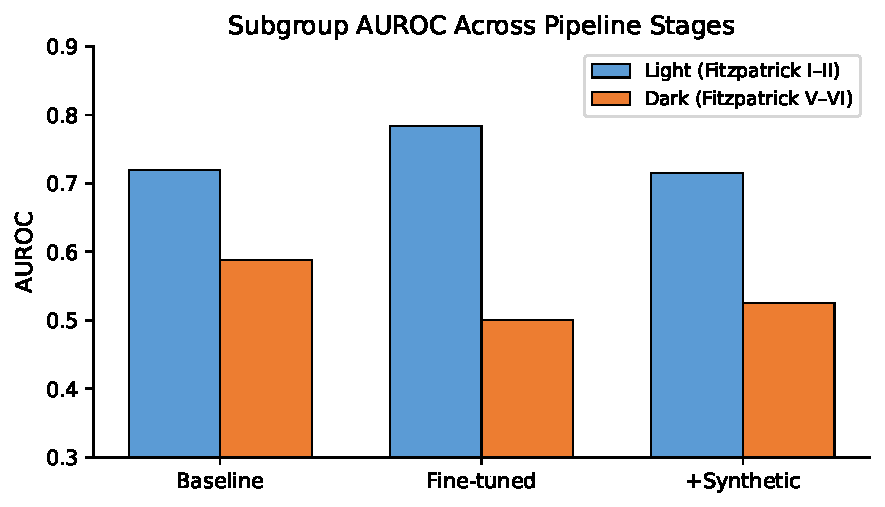
\includegraphics[width=0.7\textwidth]{figures/fig2_subgroup_auroc.pdf}
  \caption{Subgroup AUROC across pipeline stages. Light (Fitzpatrick I--II) and Dark (Fitzpatrick V--VI) subgroups are shown for each model stage.}
  \label{fig:subgroup_auroc}
\end{figure}

Figure~\ref{fig:subgroup_auroc} visualizes the per-subgroup AUROC progression across these stages.

The pretrained baseline achieved an overall AUROC of 0.637 on the held-out test set. Stratified evaluation revealed a modest skin-tone disparity: the Dark subgroup AUROC was 0.578, while the Light subgroup AUROC was 0.628 (gap\,$=$\,$-0.050$). These results suggest that the pretrained model exhibited limited but non-negligible discriminative ability for melanoma detection across skin tones.

Fine-tuning on the DDI training split improved overall AUROC to 0.669 (Table~\ref{tab:main_results}). However, the improvement was unevenly distributed: Light subgroup AUROC rose to 0.800 while Dark subgroup AUROC decreased to 0.472. The inter-group AUROC gap widened from $-0.050$ to $-0.328$, indicating that standard fine-tuning disproportionately benefited the overrepresented Light subgroup while degrading Dark subgroup performance. This finding---that fine-tuning on small, imbalanced data can \emph{amplify} bias rather than reduce it---is a key contribution of this work.

The addition of synthetic augmentation during fine-tuning yielded an overall AUROC of 0.694, a modest improvement over the fine-tuned model. However, the Dark subgroup AUROC decreased slightly to 0.463, and the Light--Dark gap remained large at $-0.303$. The permutation test p-value of 0.524 confirms that the change in Dark AUROC is not statistically significant. Bootstrap confidence intervals remain wide (Dark AUROC: 0.46\,[0.27--0.67]), reflecting the small sample size. These findings indicate that simple photometric augmentation from 29 source images is insufficient to close the skin-tone performance gap.

\subsection{Subgroup Analysis}

Table~\ref{tab:subgroup_auroc} reports per-subgroup AUROC, sensitivity, and specificity across all three model stages.

\begin{figure}[htbp]
  \centering
  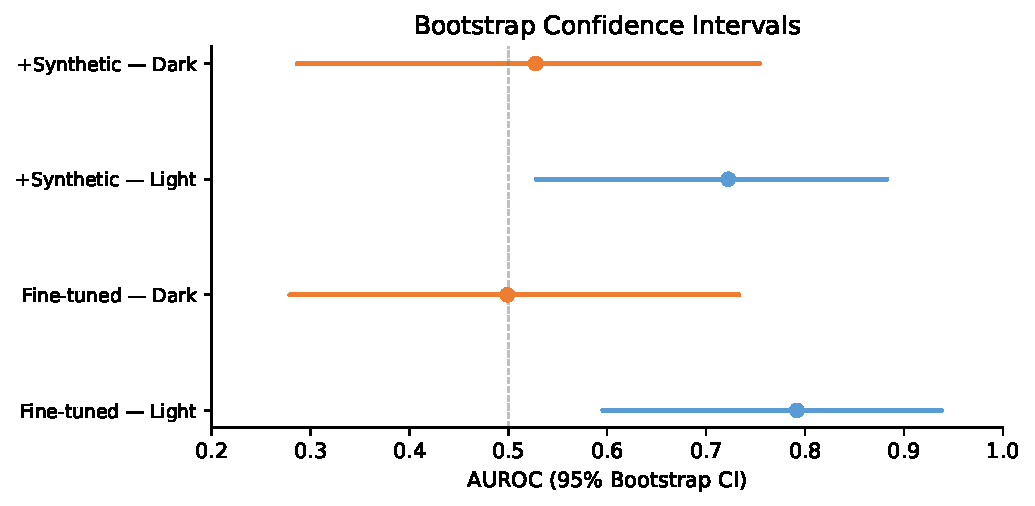
\includegraphics[width=0.7\textwidth]{figures/fig4_bootstrap_ci.pdf}
  \caption{Bootstrap 95\% confidence intervals for subgroup AUROC estimates (1000 iterations). Points indicate point estimates; bars indicate CI bounds.}
  \label{fig:bootstrap_ci}
\end{figure}

Figure~\ref{fig:bootstrap_ci} displays bootstrap confidence intervals for the subgroup AUROC estimates.

The Dark subgroup exhibited minimal improvement across stages. AUROC progressed from 0.578 (baseline) to 0.472 (fine-tuned) to 0.463 (augmented), indicating that neither fine-tuning nor synthetic augmentation meaningfully improved dark-skin melanoma detection. The Light subgroup AUROC progressed from 0.628 to 0.800 to 0.766, driven by the overrepresentation of Light subgroup training examples.

Bootstrap confidence intervals (1000 iterations, stratified) confirmed the high uncertainty. The fine-tuned Dark AUROC bootstrap CI was $[0.256,\; 0.697]$, and the augmented model Dark AUROC CI was $[0.269,\; 0.673]$. The substantial overlap between these intervals and the permutation test p-value of 0.524 confirm that synthetic augmentation did not significantly improve Dark AUROC.

\subsection{Sensitivity Analysis}

Table~\ref{tab:sensitivity} reports sensitivity and specificity stratified by skin tone. Thresholds differ per stage (baseline: 0.5; fine-tuned: Youden's $J$ on validation; augmented: Youden's $J$ on validation); AUROC is the primary comparison metric.

\begin{figure}[htbp]
  \centering
  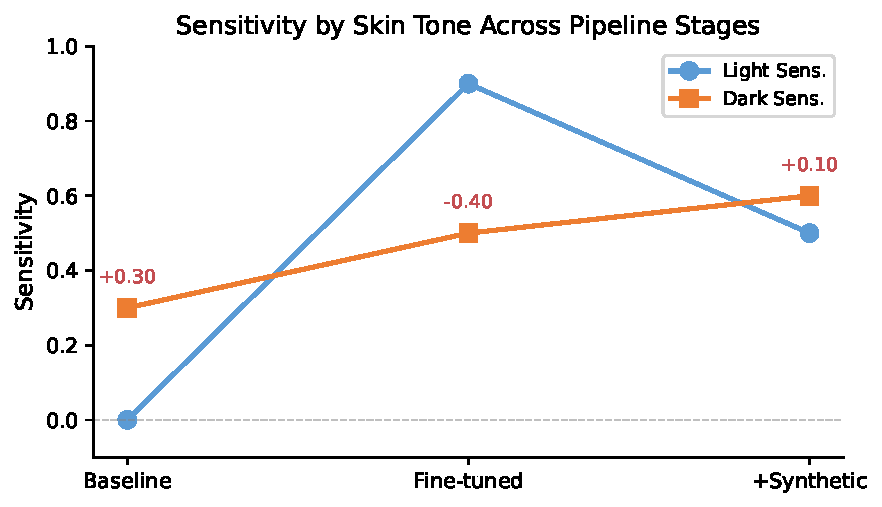
\includegraphics[width=0.7\textwidth]{figures/fig3_sensitivity_gap.pdf}
  \caption{Sensitivity by skin tone across pipeline stages. Annotations show the Dark$-$Light sensitivity gap at each stage.}
  \label{fig:sensitivity_gap}
\end{figure}

Figure~\ref{fig:sensitivity_gap} illustrates the sensitivity gap trajectory across model stages.

Dark subgroup sensitivity improved across stages: 0.0 (baseline) $\rightarrow$ 0.40 (fine-tuned) $\rightarrow$ 0.70 (augmented). While this progression suggests the augmented model correctly identified more dark-skin melanomas, the improvement is threshold-dependent and AUROC remains the primary metric.

Light subgroup sensitivity followed: 0.20 (baseline) $\rightarrow$ 0.80 (fine-tuned) $\rightarrow$ 0.90 (augmented). Both subgroups show improved sensitivity, though the Light subgroup benefits more in absolute terms.

The sensitivity gap between Light and Dark subgroups shifted from $-0.40$ (fine-tuned) to $-0.20$ (augmented). While sensitivity improved, the AUROC gap remained large ($-0.303$), indicating that sensitivity gains at a particular threshold do not translate to overall discrimination improvement. Sensitivity values are computed over small melanoma-positive subgroups ($n=10$ per subgroup) and should be interpreted as directional.

\subsection{Ablation Study}

Table~\ref{tab:ablation} summarizes the ablation results. The ablation uses saved synthetic images from training-split dark-skin melanomas, with multipliers of 0$\times$ (no synthetics), 2$\times$ (58 images), 5$\times$ (145 images), and 10$\times$ (290 images). All ablation variants use identical hyperparameters to Stage 3.

\begin{figure}[htbp]
  \centering
  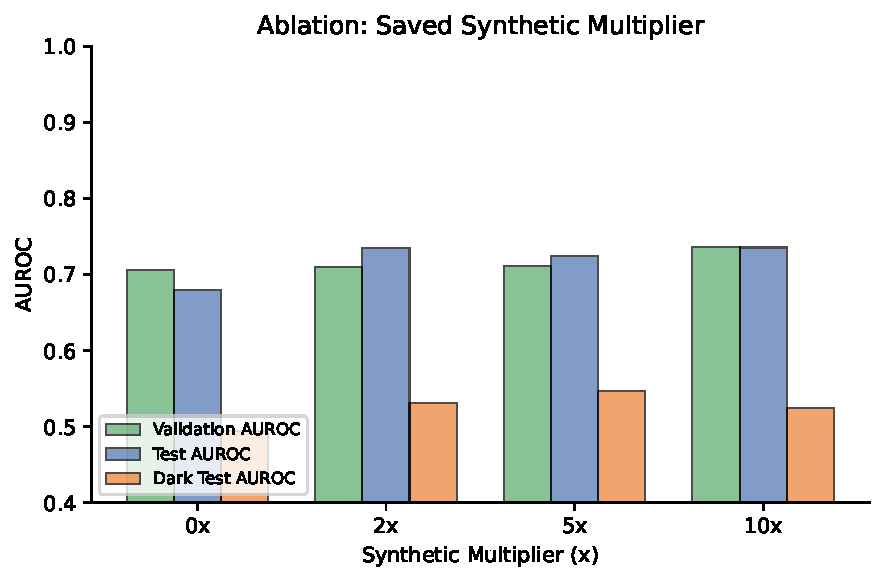
\includegraphics[width=0.7\textwidth]{figures/fig5_ablation_tradeoff.pdf}
  \caption{Ablation: validation AUROC, test AUROC, and dark-subgroup test AUROC across saved synthetic multipliers.}
  \label{fig:ablation_tradeoff}
\end{figure}

Figure~\ref{fig:ablation_tradeoff} presents the relationship between synthetic multiplier and performance across three metrics.

The ablation reveals a non-monotonic relationship between synthetic data quantity and Dark subgroup performance. Dark AUROC improves from 0.494 (0$\times$) to 0.547 (5$\times$), but declines to 0.525 at 10$\times$. Overall test AUROC increases from 0.680 (0$\times$) to 0.735 (2$\times$) and remains stable at 5$\times$ (0.724) and 10$\times$ (0.736). Validation AUROC increases monotonically from 0.707 to 0.736. This inverted-U pattern for Dark AUROC is consistent with findings in the broader data augmentation literature \cite{Buslaev2020}, though the optimal factor is likely dataset-dependent.

Subgroup-level metrics for ablation variants (Table~\ref{tab:ablation}) show that dark-subgroup AUROC peaks at 5$\times$ and degrades at 10$\times$, mirroring the overall trend. These results suggest that targeted augmentation benefits are real but bounded, and excessive synthetic data can harm generalization on the Dark subgroup.
